\section{Shannon's Answer: The Capacity of the Binary Symmetric Channel}

Section 2 showed how a finite code can trade rate for distance. This raises the question: What is the best possible trade-off? In other words, what is the maximum rate we can achieve while still communicating reliably?

Reliability in this context is a property of a family of codes: the probability of a block-decoding error approaches zero as the codeword length $n$ grows. For a $\operatorname{BSC}(p)$ with $p<1/2$, repeating a single bit more and more times is reliable in this sense, but its rate approaches zero. We want to know whether reliable families of codes can instead maintain a positive rate. Shannon's answer for the BSC is the destination of this section.

Suppose we use a $\operatorname{BSC}(p)$ $n$ times, where $n$ is large. An encoder chooses a codebook $\mathcal{C}$ containing $|\mathcal{C}|=2^k$ codewords from the $2^n$ possible binary strings, giving rate
\begin{equation}
R=\frac{k}{n}=\frac{\log_2|\mathcal{C}|}{n}.
\label{eq:chapter-three-rate}
\end{equation}

\begin{smjtheorem}[Simplified noisy-channel coding theorem for the BSC]{thm:bsc-coding-simplified}
For a $\operatorname{BSC}(p)$ with $0\leq p<1/2$, the capacity is $C_{\mathrm{BSC}}=1-h_2(p)$, where the binary entropy function $h_2(p)$ will be defined and motivated in Subsection~\ref{subsec:binary-entropy}. Then:
\begin{enumerate}
    \item If $R<C_{\mathrm{BSC}}$, there exists a family of increasingly long codes whose rates are at least $R$ and whose block-error probabilities approach zero.
    \item If $R>C_{\mathrm{BSC}}$, no family whose rates remain at least $R$ can have its block-error probability approach zero.
\end{enumerate}
This simplified statement makes no claim about the boundary case $R=C_{\mathrm{BSC}}$.
\end{smjtheorem}

Theorem~\ref{thm:bsc-coding-simplified} tells us what we are working toward. To see why this particular threshold appears, return to the length-$n$ output space. For a fixed $n$, increasing $R$ places more codewords into that space, while noise creates a cloud of plausible received words around each one. How many such clouds can the space hold before reliable decoding becomes impossible?

Sections 3.1--3.3 give a brief proof sketch rather than a complete proof of Shannon's theorem. Their purpose is to explain where the BSC capacity formula comes from. The argument has three steps:
\begin{enumerate}
    \item Determine which noise patterns are typical when $n$ is large. These patterns form the high-probability ``cloud'' around a transmitted codeword.
    \item Count the typical patterns in one cloud. The binary entropy function $h_2(p)$, defined in Subsection~\ref{subsec:binary-entropy}, will show that there are roughly $2^{nh_2(p)}$ of them.
    \item Compare the size of one cloud with the $2^n$ possible received words. This packing comparison suggests how many distinguishable codewords can fit and therefore which rates should be reliable.
\end{enumerate}
This calculation will predict the threshold $1-h_2(p)$ and give the main intuition behind both sides of Shannon's result. It is not by itself a rigorous proof: finite noise clouds may overlap, rare noise patterns remain possible, and an existence argument must show that suitable codebooks can actually be chosen. The theorem above states the result we are trying to understand; after the sketch, Subsection~\ref{subsec:general-channels} introduces the language needed to express channel capacity beyond the BSC.

\subsection{What Typical Noise Looks Like}

The first step is to describe the likely noise cloud around one transmitted codeword. For each channel use, let $Z_i=1$ if the $i$th bit is flipped and $Z_i=0$ otherwise. The BSC assumptions tell us that
\begin{equation}
Z_1,\ldots,Z_n\ \text{are independent},
\qquad
Z_i\sim\operatorname{Bern}(p).
\label{eq:bsc-noise-assumptions}
\end{equation}
The total number of flips is
\begin{equation}
K_n=Z_1+\cdots+Z_n,
\label{eq:total-bsc-flips}
\end{equation}
which has a binomial distribution and expected value $\mathbb{E}[K_n]=np$. This does not mean that exactly $np$ bits will flip. Instead, the law of large numbers says that the fraction $K_n/n$ becomes increasingly concentrated near $p$. For every fixed $\varepsilon>0$,
\begin{equation}
\Pr\left(\left|\frac{K_n}{n}-p\right|>\varepsilon\right)
\longrightarrow0
\qquad\text{as }n\longrightarrow\infty.
\label{eq:noise-concentration}
\end{equation}

We will call a noise vector $\mathbf{z}\in\{0,1\}^n$ \emph{typical} when its fraction of $1$s is close to $p$. More precisely, for a chosen tolerance $\varepsilon$, define
\begin{equation}
\mathcal{T}_{\varepsilon}^{(n)}
=\left\{\mathbf{z}\in\{0,1\}^n:
\left|\frac{\operatorname{wt}(\mathbf{z})}{n}-p\right|
\leq\varepsilon\right\}.
\label{eq:typical-noise-set}
\end{equation}
Equation~\eqref{eq:noise-concentration} says that the actual BSC noise lies in this set with probability approaching $1$. Thus a transmitted word $\mathbf{x}$ is very likely to produce an output in the translated set $\mathbf{x}\oplus\mathcal{T}_{\varepsilon}^{(n)}$. Rare patterns outside this region remain possible, but their total probability becomes small.

\begin{figure}[htbp]
    \centering
    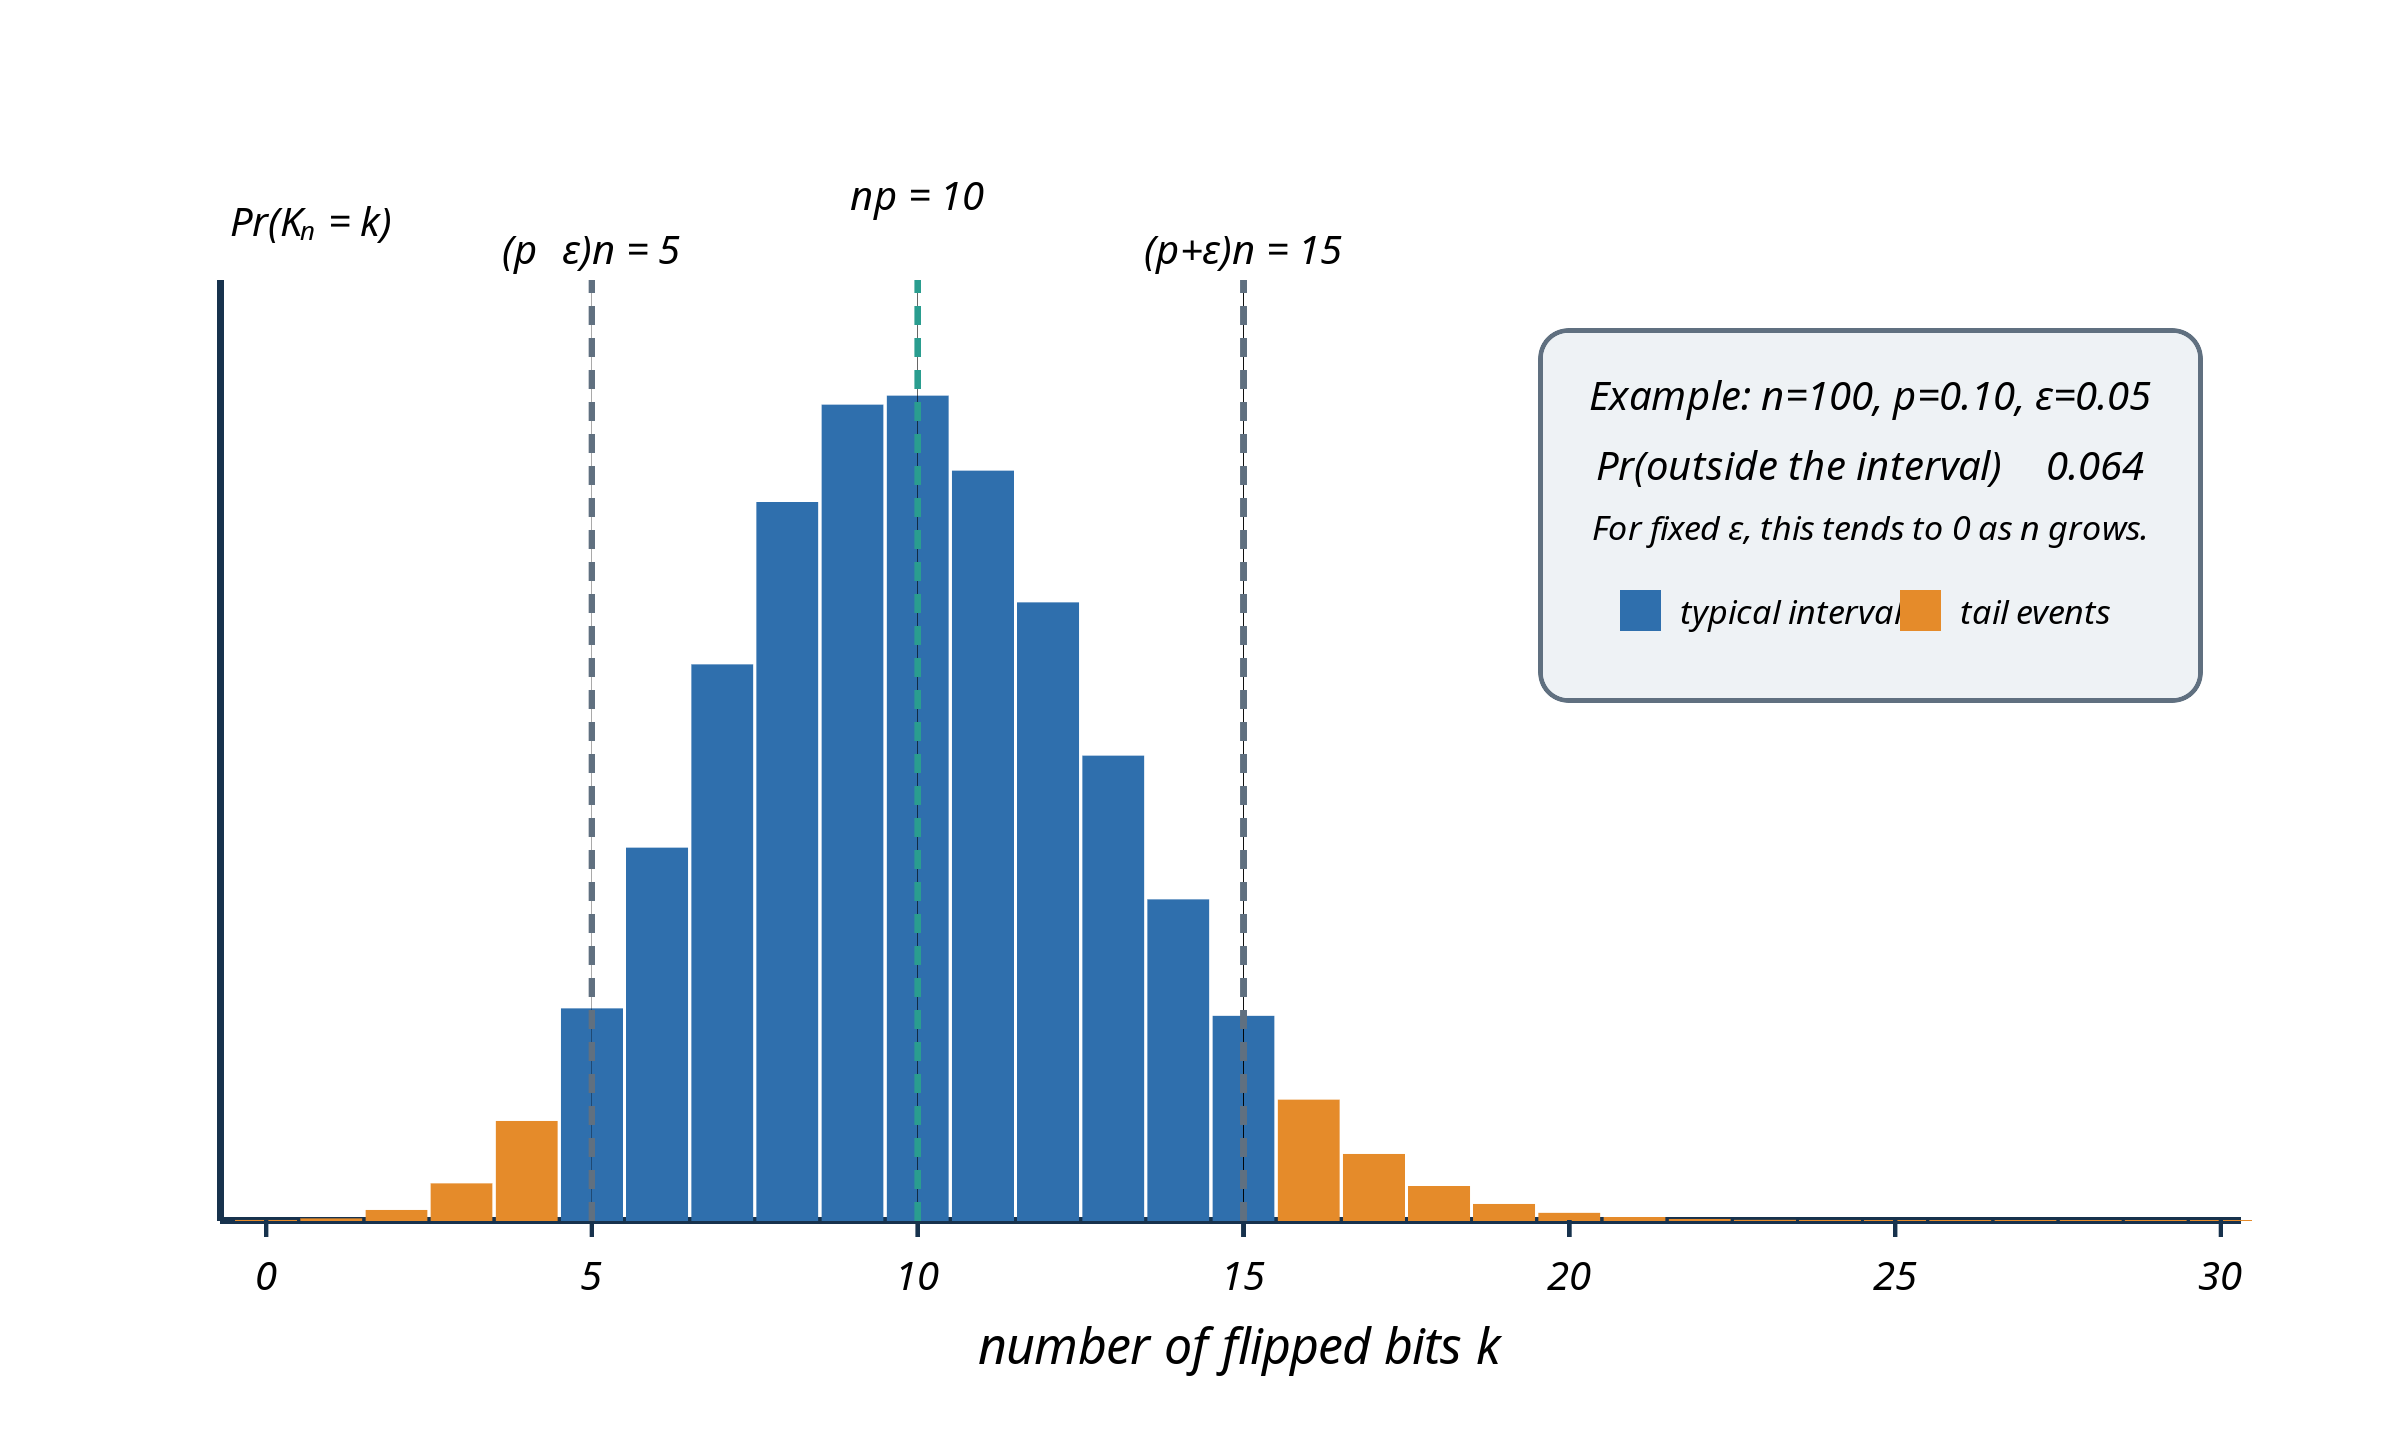
\includegraphics[width=0.9\linewidth]{assets/binomial_typical_set.png}
    \caption{For $n=100$ and $p=0.10$, the binomial number of flipped bits $K_n$ concentrates near its mean $np$. The highlighted interval is $[(p-\varepsilon)n,(p+\varepsilon)n]$ with $\varepsilon=0.05$.}
    \label{fig:noise-concentration}
\end{figure}

\subsection{Counting Likely Noise Patterns: Binary Entropy}
\label{subsec:binary-entropy}

The first step told us which noise patterns make up the likely cloud around a codeword. The second step is to count them. Before doing so, it helps to attach a numerical meaning to uncertainty. If an outcome $a$ has probability $P(a)$, its \emph{self-information} is
\begin{equation}
\imath(a)=\log_2\frac{1}{P(a)}=-\log_2P(a).
\label{eq:self-information}
\end{equation}
An unlikely outcome carries more self-information because observing it is more surprising. An outcome with probability $0.99$, for example, carries little self-information because it was already strongly expected.

The average self-information of a random variable is its \emph{entropy}. For example, suppose you flip a fair coin once. Let $X$ represent the coin outcome, with $X=1$ for heads and $X=0$ for tails. A fair coin therefore has the Bernoulli distribution $X\sim\operatorname{Bern}(1/2)$, meaning
\begin{equation}
\Pr(X=1)=0.5,
\qquad
\Pr(X=0)=0.5.
\label{eq:fair-coin-distribution}
\end{equation}
Its entropy is the probability-weighted average of the two outcomes' self-information:
\begin{equation}
H(X)=-\big[0.5\log_2 0.5+0.5\log_2 0.5\big]
=1\text{ bit}.
\label{eq:fair-coin-entropy}
\end{equation}
Thus, before the toss is observed, the fair coin has $1$ bit of uncertainty.

If the coin is biased, say
\begin{equation}
\Pr(X=1)=0.9,
\qquad
\Pr(X=0)=0.1,
\label{eq:biased-coin-distribution}
\end{equation}
then its entropy is
\begin{equation}
H(X)=-\big[0.9\log_2 0.9+0.1\log_2 0.1\big]
\approx0.47\text{ bits}.
\label{eq:biased-coin-entropy}
\end{equation}
The biased coin has less uncertainty because one outcome is much more predictable.

The BSC noise indicator is also a Bernoulli random variable: it equals $1$ with probability $p$ and $0$ with probability $1-p$. Applying the same average-surprise calculation gives the \emph{binary entropy function}
\begin{equation}
h_2(p)=-p\log_2p-(1-p)\log_2(1-p),
\label{eq:binary-entropy}
\end{equation}
where $0\log_2 0$ is interpreted as $0$. Figure~\ref{fig:binary-entropy} shows how the binary entropy changes with $p$.

\begin{figure}[htbp]
    \centering
    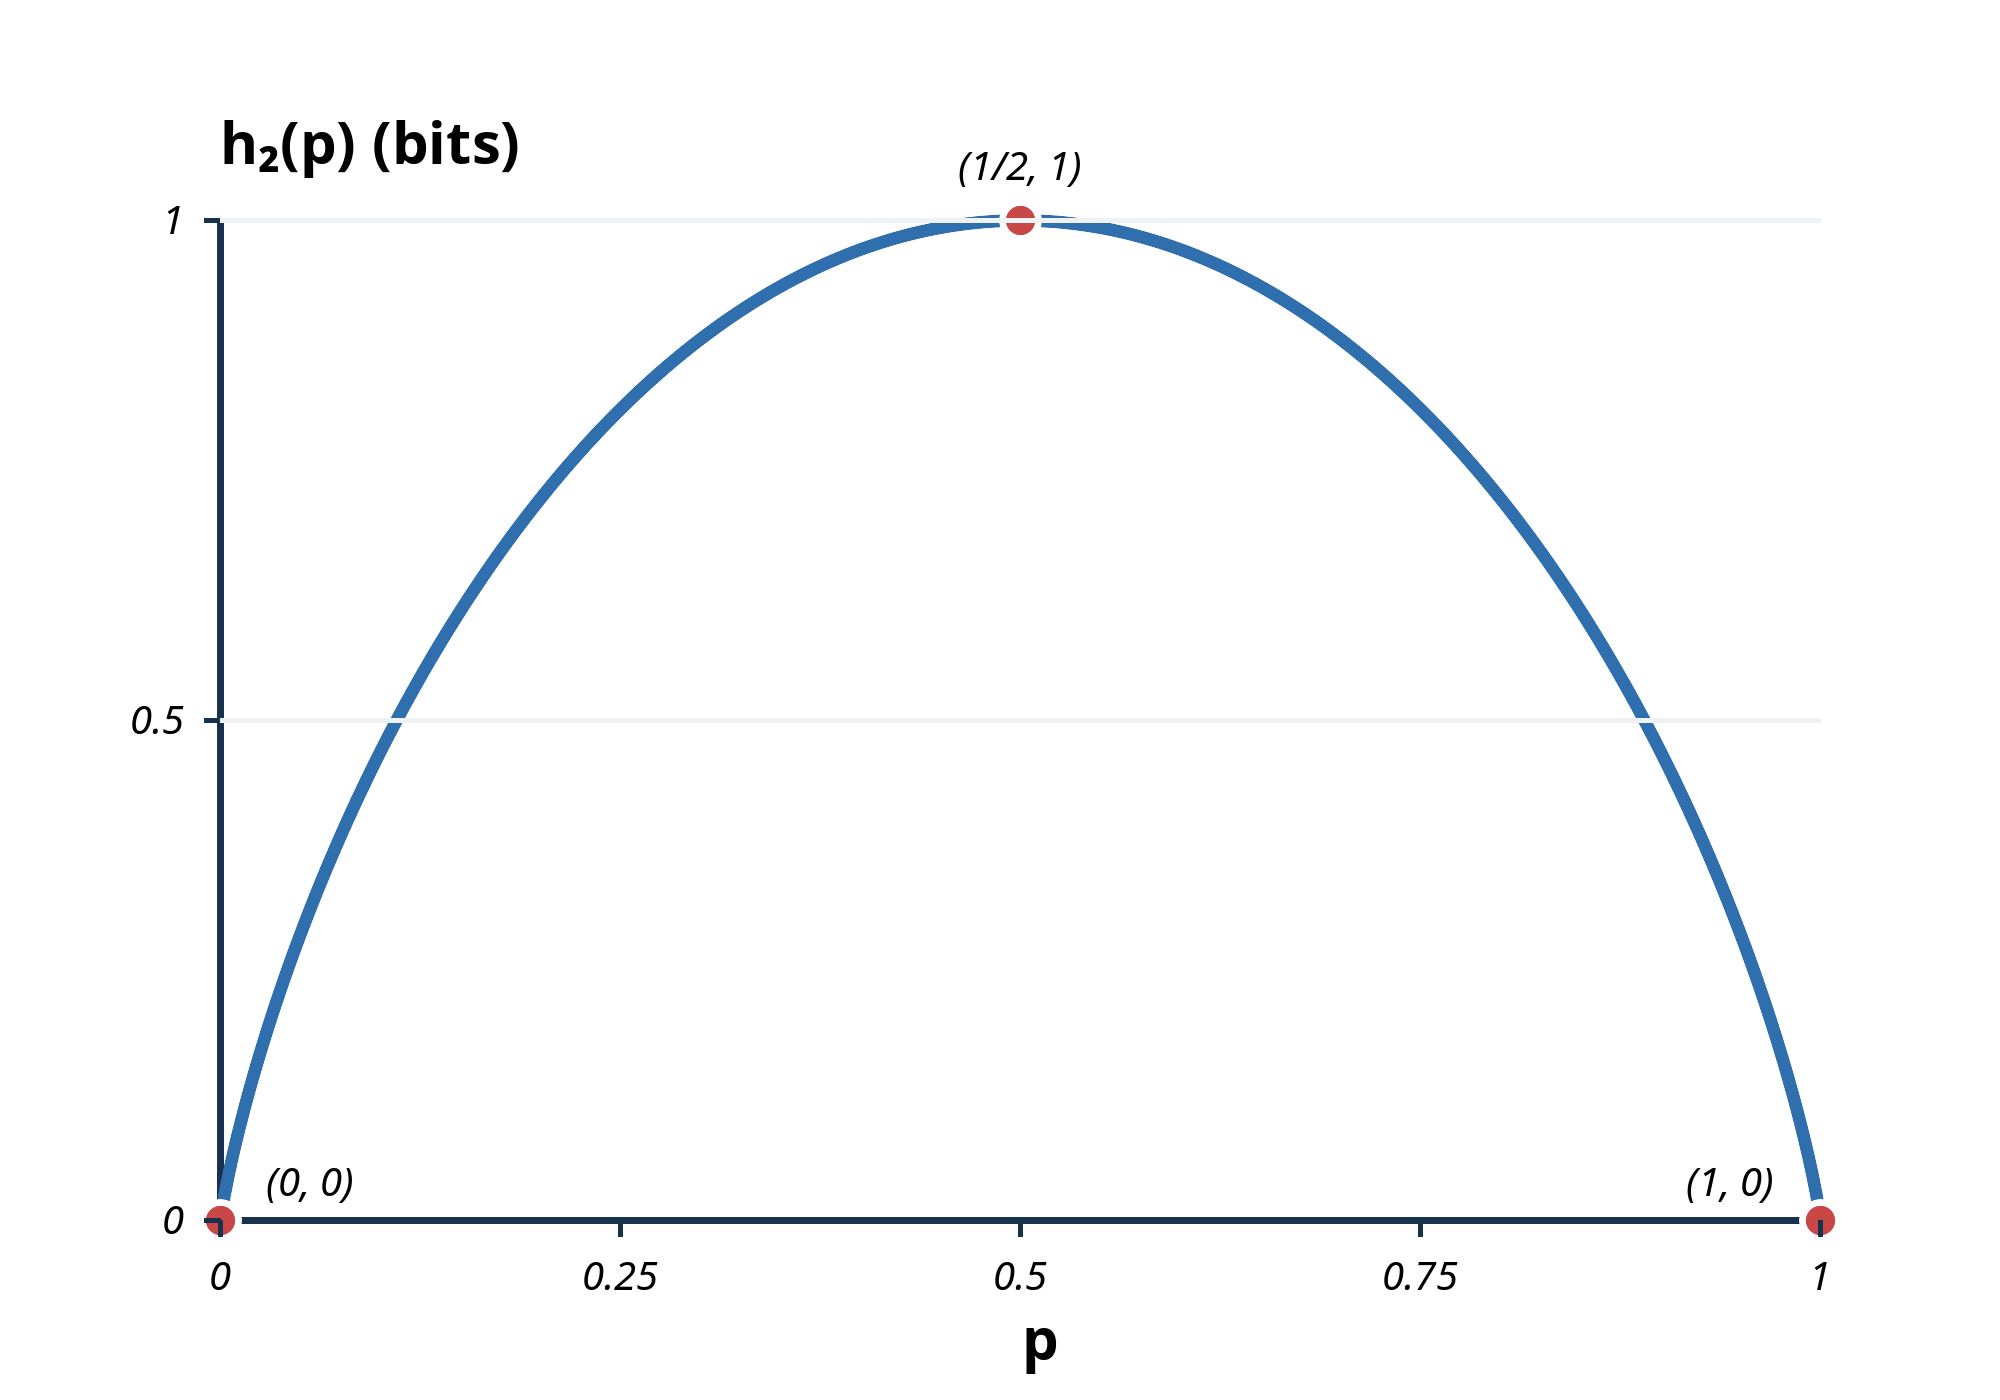
\includegraphics[width=0.72\linewidth]{assets/binary_entropy.png}
    \caption{The binary entropy function $h_2(p)$, which reaches its maximum value $1$ at $p=1/2$.}
    \label{fig:binary-entropy}
\end{figure}

We can now return to the counting problem. A length-$n$ noise vector with exactly $w$ flips can be formed by choosing which $w$ positions contain a $1$. There are
\begin{equation}
\binom{n}{w}
\label{eq:weight-w-noise-count}
\end{equation}
such vectors. When $w$ is close to $np$, Stirling's approximation---an approximation for factorials when the numbers involved are large---gives, on the exponential scale,
\begin{equation}
\binom{n}{\lfloor np\rfloor}\approx2^{nh_2(p)}.
\label{eq:entropy-counting}
\end{equation}
Here $\lfloor np\rfloor$ rounds $np$ down to a whole number so that it can represent a possible number of flipped bits. For a small tolerance $\varepsilon$, the exponential growth rate of the entire typical set is close to $h_2(p)$, and it approaches $h_2(p)$ as the tolerance is tightened. Factors that grow only polynomially with $n$ are hidden by the approximation. The important conclusion is that one codeword has roughly $2^{nh_2(p)}$ likely noise patterns around it on the exponential scale.



\subsection{From Counting to the BSC Capacity}

The first two steps showed that one codeword has roughly $2^{nh_2(p)}$ likely outputs after passing through the BSC; that is, its likely-output cloud has roughly this many elements. To see why, fix a codeword $\mathbf{c}\in\mathcal{C}$. Equation~\eqref{eq:entropy-counting}, together with the typical-set discussion following it, shows that there are roughly $2^{nh_2(p)}$ relevant noise patterns $\mathbf{z}$ on the exponential scale. Each one produces a received word $\mathbf{y}=\mathbf{c}\oplus\mathbf{z}$. Thus $2^{nh_2(p)}$ is the approximate size of the likely-output cloud around one codeword.

The final step compares all these clouds with the entire output space. The factor $|\mathcal{C}|$ is the number of valid codewords, $2^{nh_2(p)}$ is the approximate number of likely outputs per codeword, and $2^n$ is the total number of length-$n$ received words. If the likely-output clouds are to remain distinguishable, their combined size should not exceed the available output space. This gives the packing estimate
\begin{equation}
|\mathcal{C}|\,2^{nh_2(p)}\lesssim2^n.
\label{eq:typical-cloud-packing}
\end{equation}
Here $\lesssim$ reminds us that this is an exponential-scale estimate rather than an exact finite-length inequality. If the left-hand side were substantially larger than $2^n$, many likely-output clouds would have to overlap, making different transmitted codewords difficult to distinguish. Solving Equation~\eqref{eq:typical-cloud-packing} for the codebook size gives
\begin{align}
|\mathcal{C}|&\lesssim\frac{2^n}{2^{nh_2(p)}}
\label{eq:codebook-cardinality-quotient}\\
&=2^{n(1-h_2(p))}.
\label{eq:codebook-cardinality-exponent}
\end{align}
Starting from Equation~\eqref{eq:codebook-cardinality-exponent}, take the base-$2$ logarithm of both sides. Because $\log_2$ is an increasing function, the direction of the estimate is preserved:
\begin{subequations}
\label{eq:bsc-capacity-derivation}
\begin{align}
\log_2|\mathcal{C}|
&\lesssim \log_2\!\left(2^{n(1-h_2(p))}\right)
\label{eq:bsc-capacity-take-log}\\
&=n(1-h_2(p)).
\label{eq:bsc-capacity-simplify-log}
\end{align}
Dividing both sides by $n$ gives
\begin{equation}
\frac{\log_2|\mathcal{C}|}{n}
\lesssim 1-h_2(p).
\label{eq:bsc-capacity-divide-by-n}
\end{equation}
Equation~\eqref{eq:chapter-three-rate} identifies the expression on the left as the code rate, so
\begin{equation}
R\lesssim 1-h_2(p).
\label{eq:bsc-capacity-rate-bound}
\end{equation}
The packing sketch therefore suggests $1-h_2(p)$ as the limiting rate. Shannon's theorem makes this prediction rigorous and identifies it as the \emph{capacity} of the $\operatorname{BSC}(p)$:
\begin{equation}
C_{\mathrm{BSC}}=1-h_2(p)
\qquad\text{bits per channel use}.
\label{eq:bsc-capacity}
\end{equation}
\end{subequations}

For example, if $p=0.1$, then
\begin{align}
C_{\mathrm{BSC}}
&=1-h_2(0.1)
\label{eq:bsc-capacity-point-one-substitution}\\
&\approx1-0.469
\label{eq:bsc-capacity-point-one-approximation}\\
&=0.531.
\label{eq:bsc-capacity-point-one-value}
\end{align}
For a block length $n=1000$, the output space contains $2^{1000}$ words and each codeword has on the order of $2^{469}$ typical noise patterns. Their ratio is approximately $2^{531}$, suggesting about $531$ message bits per $1000$ channel uses at the limiting rate. This is an asymptotic counting estimate, not a guarantee that a particular length-$1000$ code can transmit $531$ bits with negligible error.

This argument is counting intuition, not yet a proof. The Hamming balls in Section 2 described a worst-case guarantee: every pattern of up to $t$ errors had to be corrected. A typical region describes only the errors that carry almost all of the probability, and rare errors outside it are allowed to cause decoding failures. Furthermore, a rigorous coding proof does not require every finite-length typical region to be perfectly disjoint. It shows instead that their total ambiguity can be made increasingly unlikely when the rate is below the threshold.

\subsection{From the BSC to General Channels}
\label{subsec:general-channels}

The expression $1-h_2(p)$ is specific to the BSC, but Shannon's theorem applies more broadly to discrete memoryless channels. We now introduce the language that expresses how much information one random variable provides about another.

For a discrete random variable $X$, its \emph{alphabet} $\mathcal{X}$ is the set of values it can take, and $P_X(x)=\Pr(X=x)$ is the probability that it takes a particular value $x$. Its \emph{entropy} is the average self-information
\begin{equation}
H(X)=-\sum_{x\in\mathcal{X}}P_X(x)\log_2P_X(x).
\label{eq:entropy-general}
\end{equation}
Entropy measures uncertainty before an observation is made, in bits. After observing one particular output $Y=y$, the remaining uncertainty about the input is
\begin{equation}
H(X\mid Y=y)
=-\sum_{x\in\mathcal{X}}P_{X\mid Y}(x\mid y)
\log_2P_{X\mid Y}(x\mid y),
\label{eq:conditional-entropy-at-output}
\end{equation}
where $P_{X\mid Y}(x\mid y)=\Pr(X=x\mid Y=y)$ is the probability of input $x$ after output $y$ has been observed. Different outputs can leave different amounts of uncertainty. The \emph{conditional entropy} averages Equation~\eqref{eq:conditional-entropy-at-output} over every possible output $y$ in the output alphabet $\mathcal{Y}$:
\begin{equation}
H(X\mid Y)
=\sum_{y\in\mathcal{Y}}P_Y(y)H(X\mid Y=y),
\label{eq:conditional-entropy-general}
\end{equation}
where $P_Y(y)=\Pr(Y=y)$. The difference between the uncertainty before and after observing the output is the \emph{mutual information}
\begin{equation}
I(X;Y)=H(X)-H(X\mid Y).
\label{eq:mutual-information}
\end{equation}
It measures how much observing $Y$ reduces our uncertainty about $X$.

Return to the $\operatorname{BSC}(p)$ and suppose Alice uses $0$ and $1$ equally often. As Figure~\ref{fig:binary-entropy} shows, $H(X)=1$ bit. Given the output $Y$, the input equals that output with probability $1-p$ and differs from it with probability $p$. Therefore,
\begin{equation}
H(X\mid Y)=h_2(p),
\label{eq:bsc-conditional-entropy}
\end{equation}
and hence
\begin{equation}
I(X;Y)=1-h_2(p).
\label{eq:bsc-mutual-information}
\end{equation}
This reproduces the capacity suggested by our counting argument.

\begin{figure}[H]
    \centering
    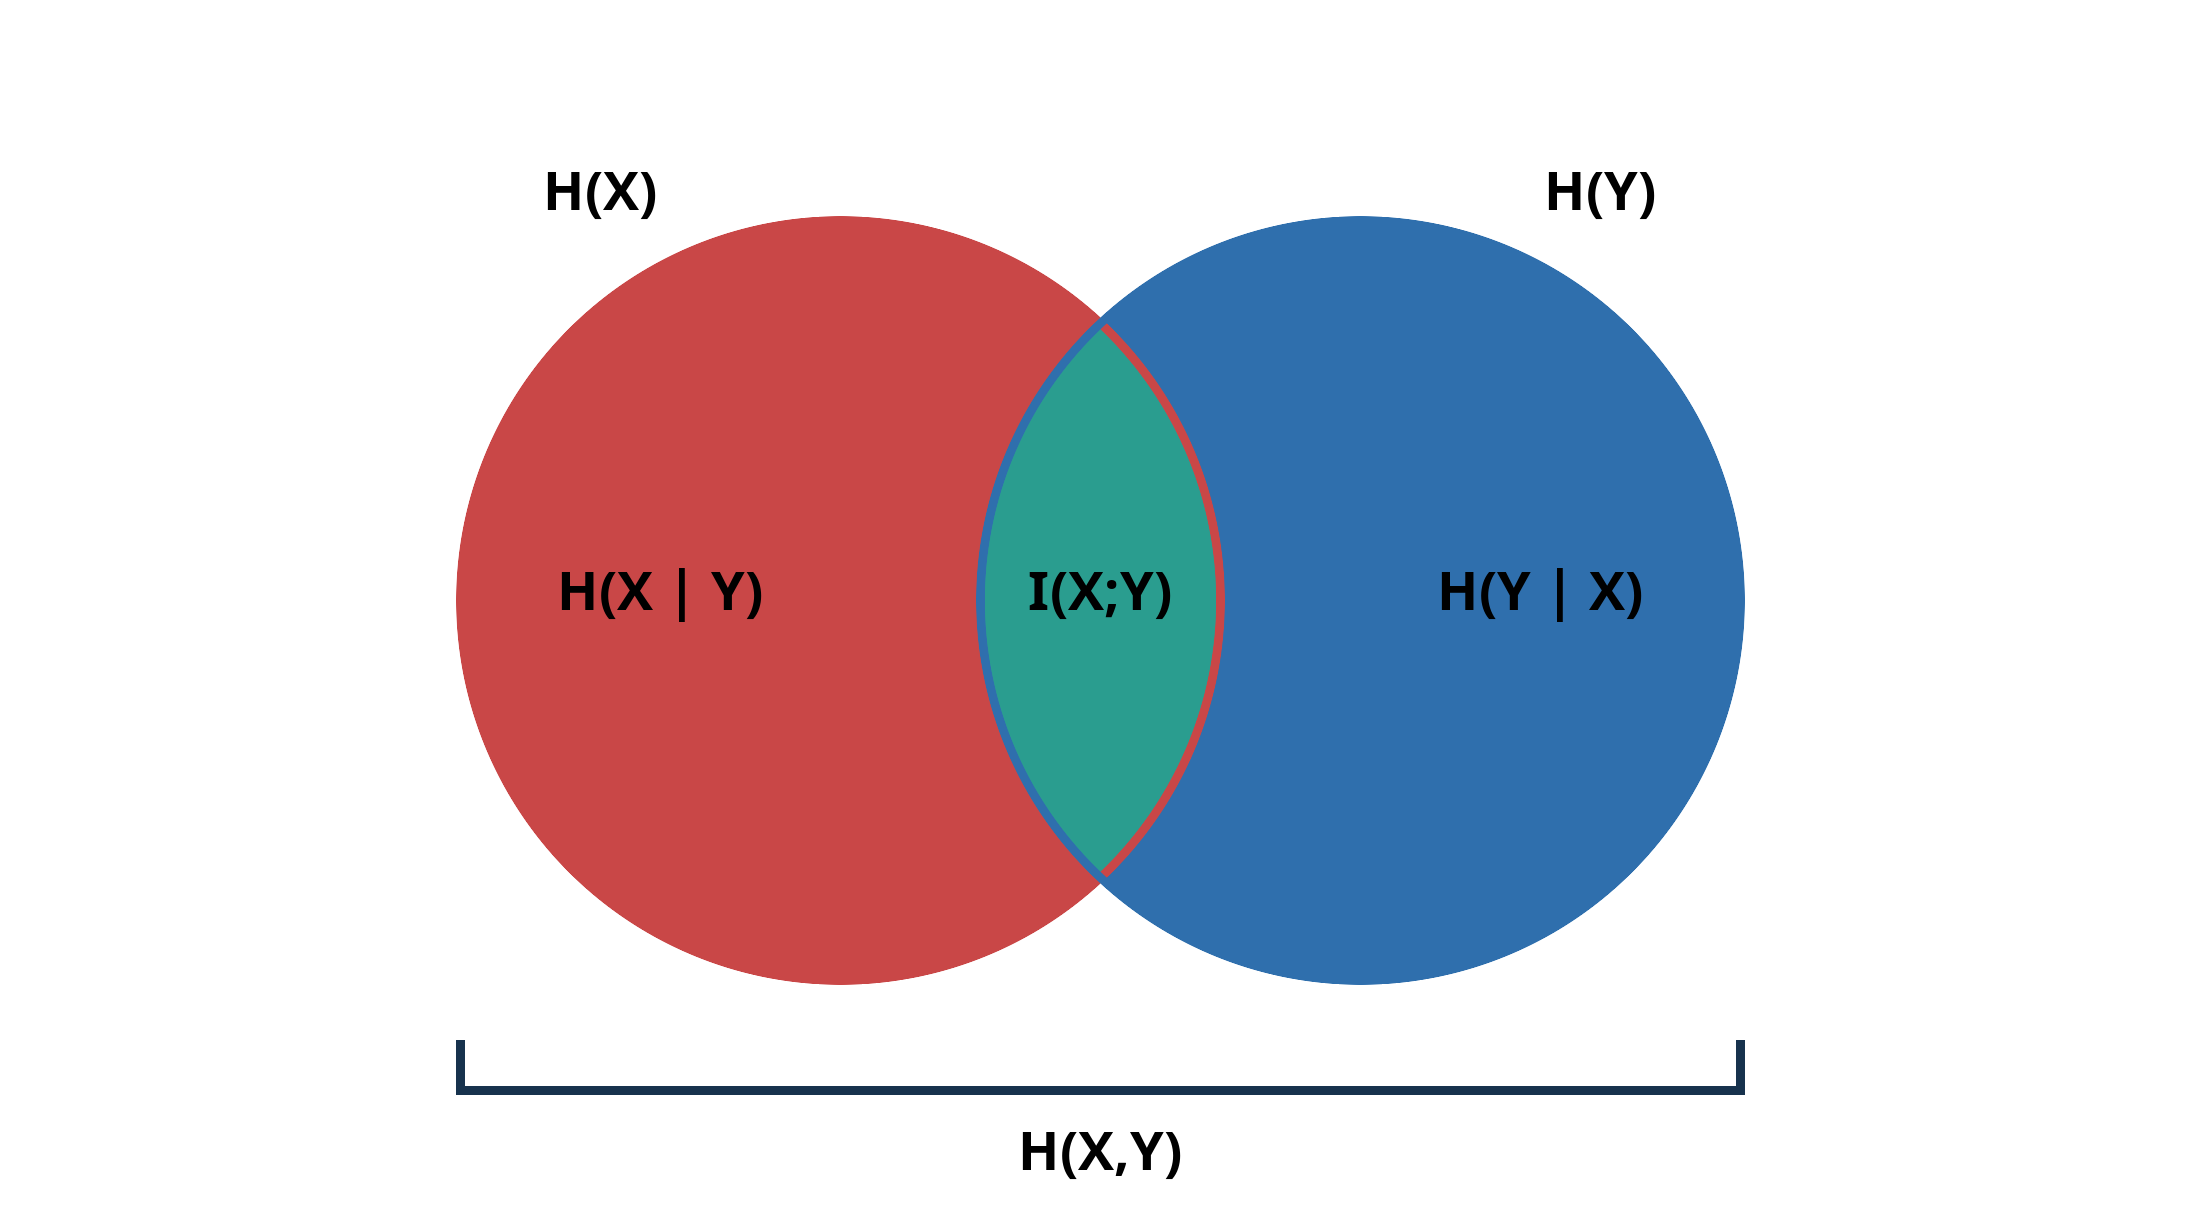
\includegraphics[width=0.6\linewidth]{assets/mutual_information_heuristic.png}
    \caption{A heuristic information diagram. The overlap represents $I(X;Y)$, while the non-overlapping portions represent $H(X\mid Y)$ and $H(Y\mid X)$. Entropy is not literally a geometric area in general.}
    \label{fig:entropy-venn}
\end{figure}

Interchanging the roles of the variables defines $H(Y\mid X)$ in the same way. Figure~\ref{fig:entropy-venn} also uses $H(X,Y)$ for the entropy of the pair $(X,Y)$ considered jointly. The polar transform will give us a reason to define joint entropy and its chain rule formally in Subsection~\ref{subsec:polar-core-idea}.

For a general discrete memoryless channel, different input distributions may carry different amounts of information. Its capacity is therefore defined by
\begin{equation}
C=\max_{P_X}I(X;Y),
\label{eq:general-channel-capacity}
\end{equation}
where the maximum is taken over all probability distributions $P_X$ on the channel input alphabet. The symmetry of the BSC makes the uniform input distribution optimal, so Equation~\eqref{eq:general-channel-capacity} reduces to $C=1-h_2(p)$ in that case.

Shannon's theorem answers a fundamental question: it tells us which communication rates are possible. However, a limit is not yet a design. Knowing that reliable codes exist below capacity does not tell Alice and Bob which code to use, how to generate its codewords, or how Bob should decode without an enormous search. We must therefore change our question. Instead of asking only, ``What rates are possible?'', we now ask, ``How can we explicitly build and efficiently decode codes that approach those rates?''
